\chapter{Molecular Dynamics}\label{ch:md}

Using the lessons learned in the previous chapter and after a reasonably successful validation of simulations (see section XX), we can use the computational parameters at a lower precision and perform Molecular Dynamics simulations in VASP. The purpose of this chapter is to outline the chosen defect structures, discuss the computational details and present how defects (interstitial or otherwise) modifies the structure and dynamics of the parent structure.

\section{Octahedral tilts}
\begin{figure}
	\centering
	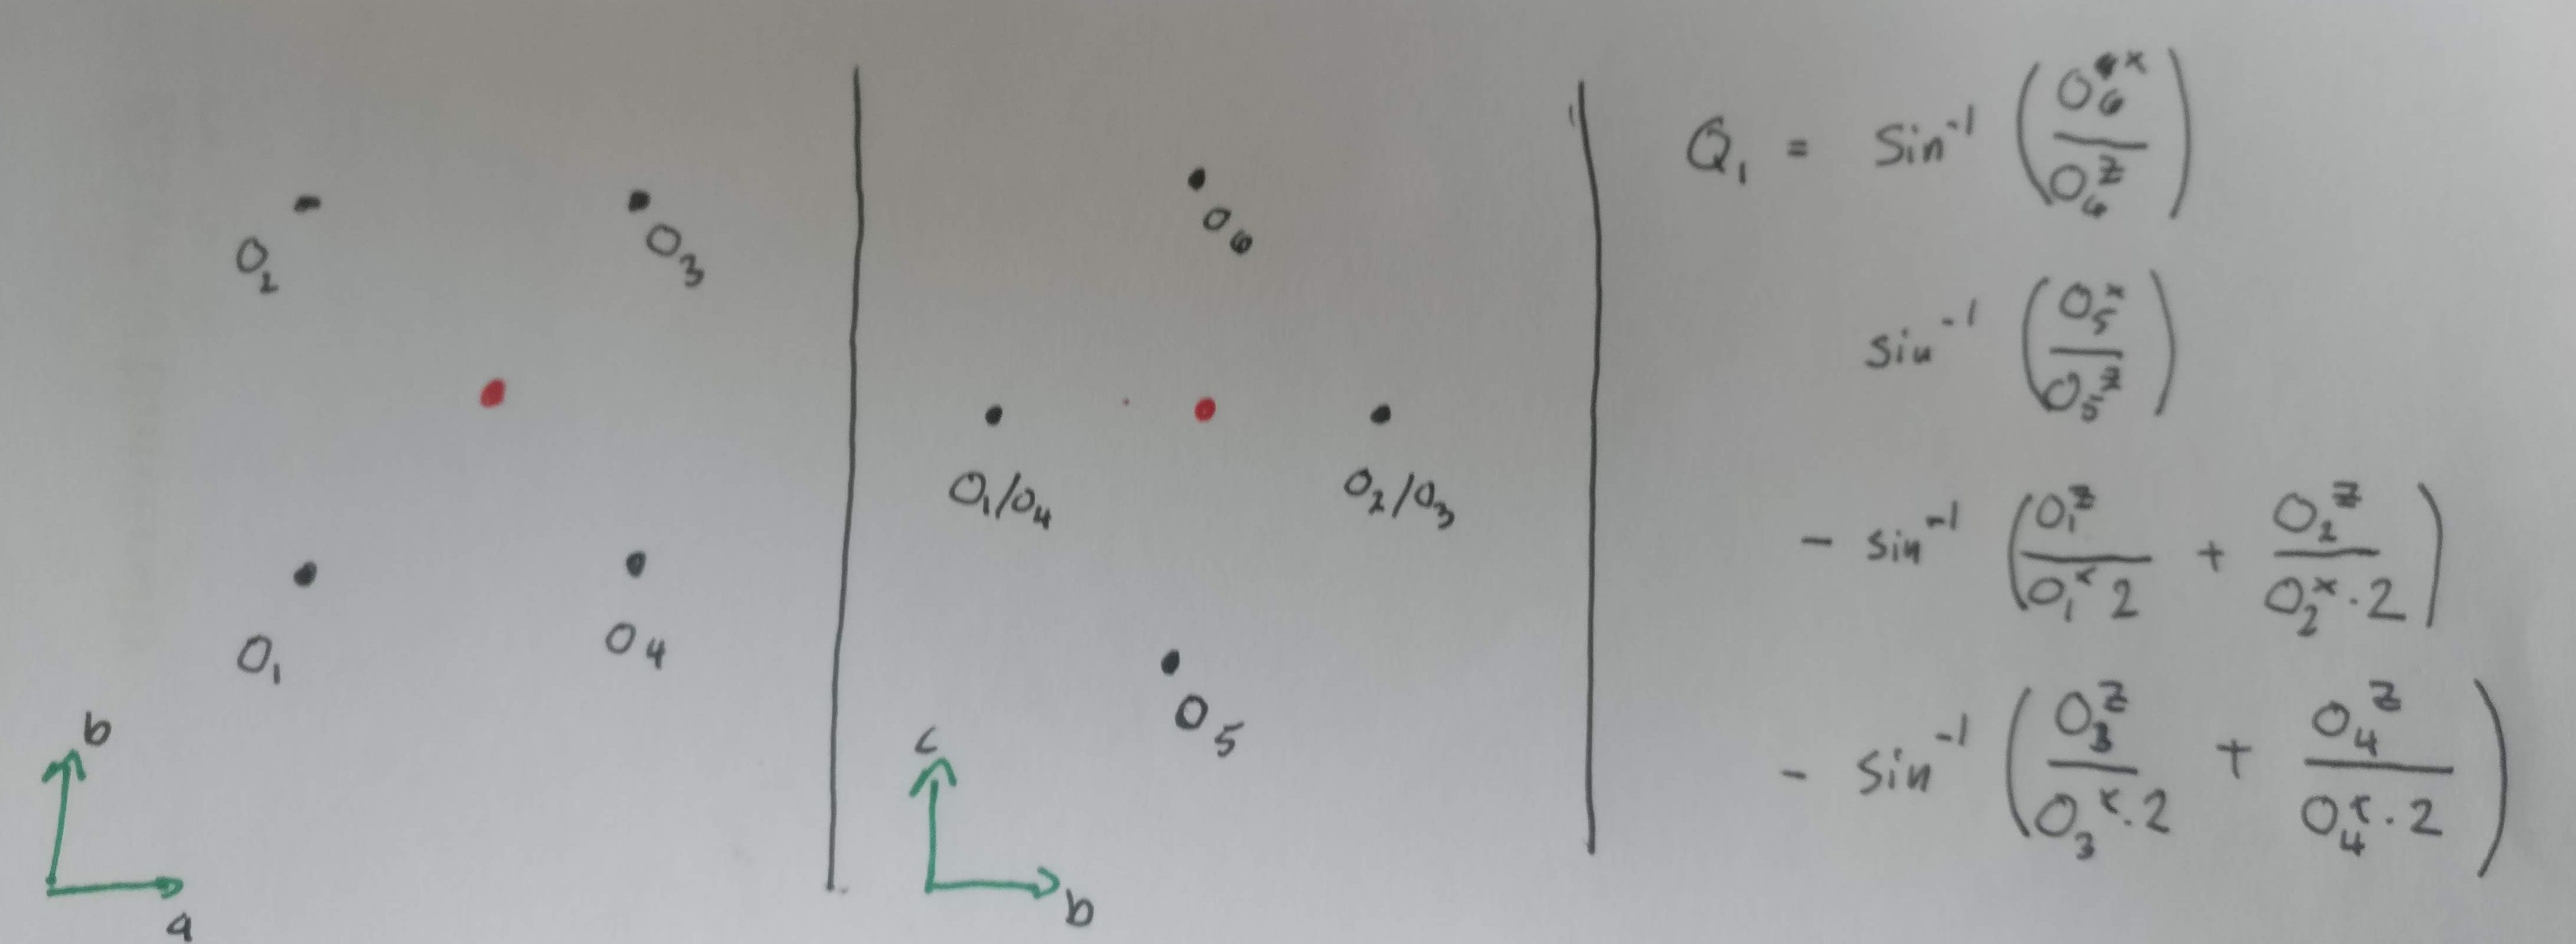
\includegraphics[width=\textwidth]{fig/md/octahedral_tilts_md.jpg}
	\caption[Finding octahedral tilts from arbitrary oxygen positions]{Finding octahedral tilts from arbitrary oxygen positions. $Q_2$ angles can be found by replacing $x$ with $y$ and `pairing up' O$_1$ with O$_4$ and O$_2$ with O$_3$.}
	\label{fig:md_octahedral_tilts}
\end{figure}

In order to obtain octahedral tilts from MD simulations where symmetry is P1, we are forced to define an average tilt. In fact, by writing which octahedra each oxygen atom (excluding interstitials) in our simulation belongs to, we can extract the $(Q_1,Q_2)$ tilt as seen from that oxygen. Since the tilts alternate, each tilt belongs to one of four symmetries with respect to $(Q_1,Q_2)$: (+,+), (+,-), (-,+), (-,-). In practice, we analyse the initial $t=0$ structure with the following steps for each Cu atom in the supercell:

\begin{enumerate}
	\item Record the position of the Cu atom
	\item Find apical oxygens by searching for O with a Cu-O distance less than $r = (1,1,2.7) \, \SI{}{\angstrom}$
	\item Find equatorial oxygens by searching for O with a Cu-O distance less than $r = (2.1,2.1,1) \, \SI{}{\angstrom}$
	\item Determine the $Q_1$, $Q_2$ tilt as seen from each of the 6 oxygen atoms in the list.
	\item Apply the symmetry operations.
	\item Save all 4 ($Q_1$, $Q_2$) value pairs.
\end{enumerate}

\noindent Step 4 is performed by first converting fractional coordinates to real-space coordinates and then finding angles as outlined in Figure \ref{fig:md_octahedral_tilts}. The symmetry operations in step 5 is a matrix with 8 columns corresponding to the 8 tilt values and a number of rows equal to the number of octahedra -- 16 in the case of our $2 \times 2 \times 2$ supercell. Each element of the matrix is either +1 or -1, where -1 will reverse the tilt direction and +1 will keep it as-is. The matrix can be generated by examining the output of the starting structure (which has the correct space group symmetry) and then constructing the matrix such that all tilts agree. While the same result can be archived by manually assigning the different atoms of our manageable supercell, this methodology allows the code to eventually be expanded to other systems since we can set up arbitrary local coordinate systems.

After having performed this analysis, we can apply the same operations to every time step and obtain statistics about the time-evolution of the octahedral tilts in our system. This is similar to the Positional Recurrence Maps (PRM) methodology \cite{Piovano2016} that has been used to extract dynamical information about the apical oxygen in Nd$_2$NiO$_{4+\delta}$ \cite{Perrichon2015}.

\section{Molecular Dynamics}
\[ T = \frac{1}{3 k_\text{B} (N_\text{ions}-1)} \sum_n M_n |\bm{v}_n|^2 \]
\todo[inline]{in progress... Data from LTO and LTT exists...}

\begin{figure}
	\centering
	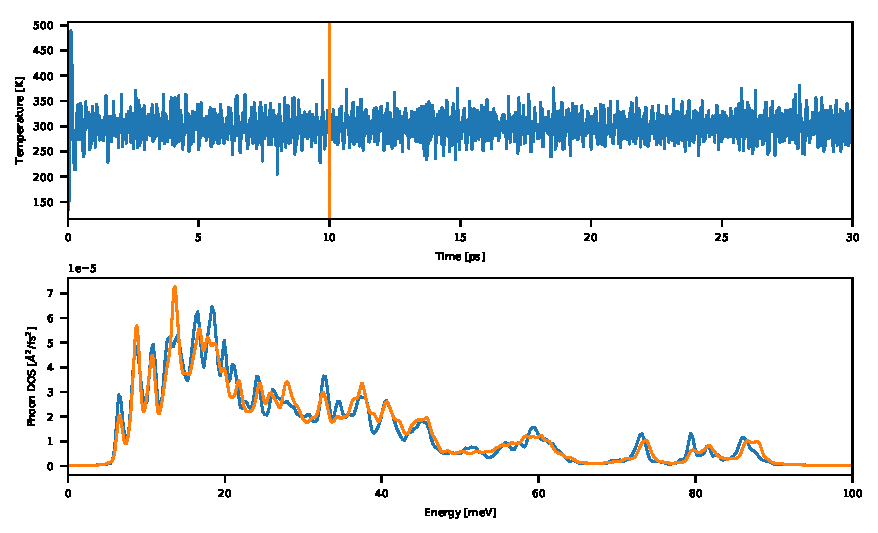
\includegraphics[width=\textwidth]{fig/md/stitch.pdf}
	\caption[stitched md runs]{sticthed md runs and comparison}
	\label{fig:stitch}
\end{figure}

\begin{figure}
	\centering
	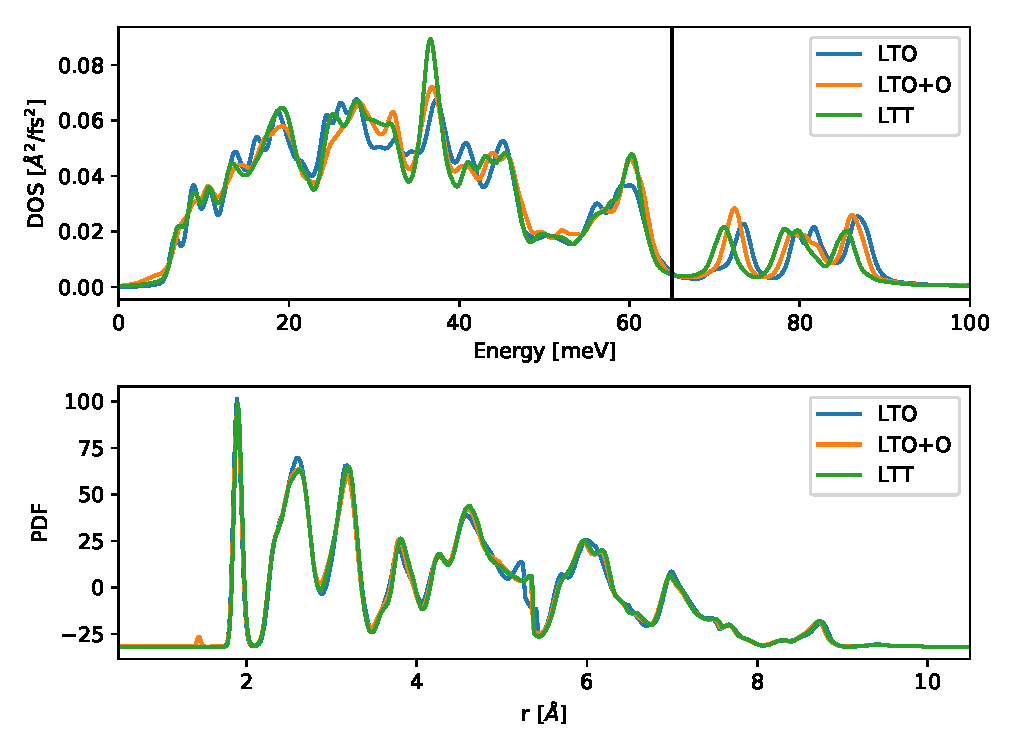
\includegraphics[width=\textwidth]{fig/md/lto_ltt_ltoo_comparison.pdf}
	\caption[MD: DOS and PDF]{MD: DOS and PDF}
	\label{fig:dos_pdf}
\end{figure}

\begin{figure}[]
	\centering
	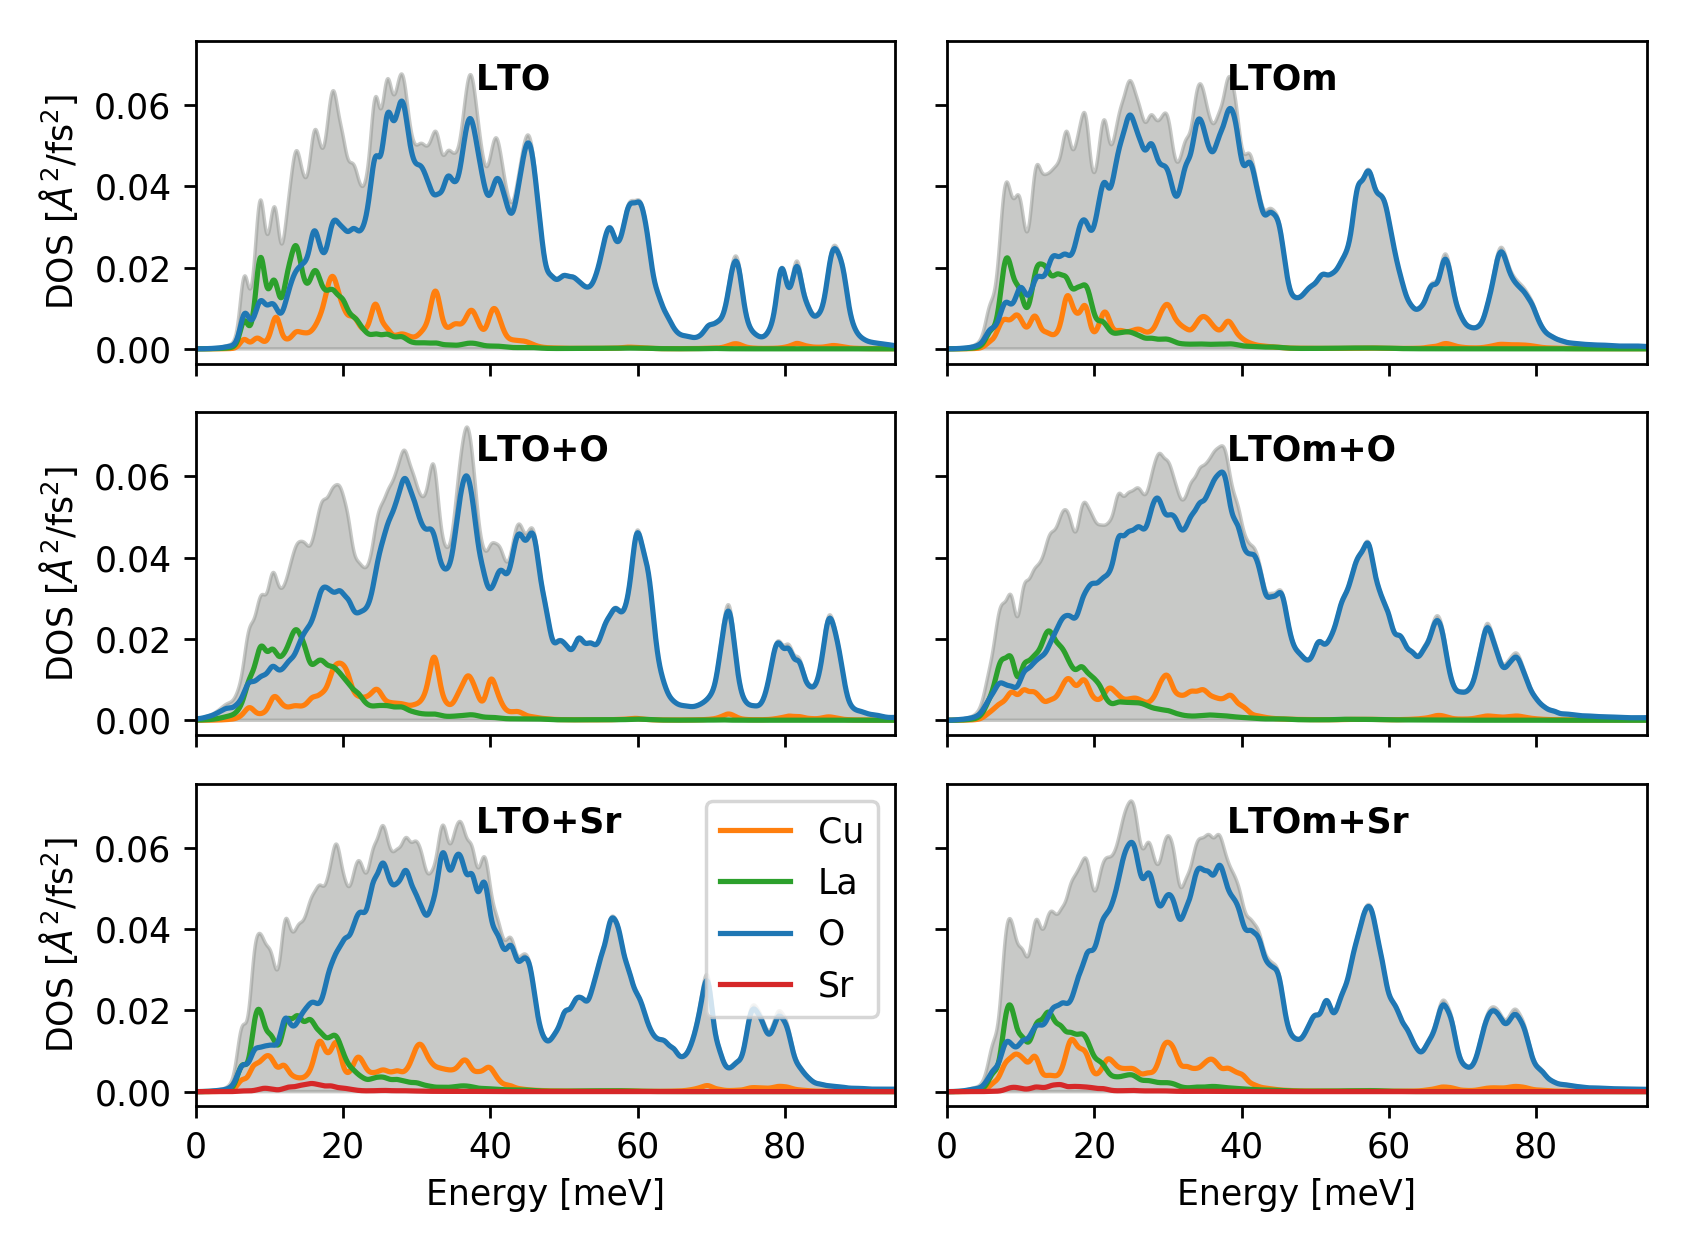
\includegraphics[width=\textwidth]{fig/md/lto_defect_comparison.png}
	\caption[LTO MD DOS: Defect comparision]{LTO MD DOS: Defect comparision}
	\label{fig:lto_md_defect_comparison}
\end{figure}

\begin{figure}
	\centering
	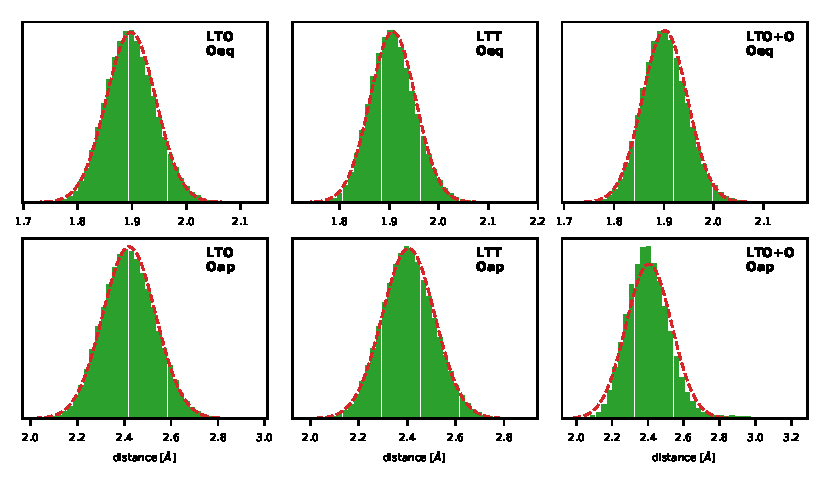
\includegraphics[width=\textwidth]{fig/md/dist_hist.pdf}
	\caption[MD: distance histograms]{MD: distance histograms}
	\label{fig:md_distances}
\end{figure}

\begin{figure}
	\centering
	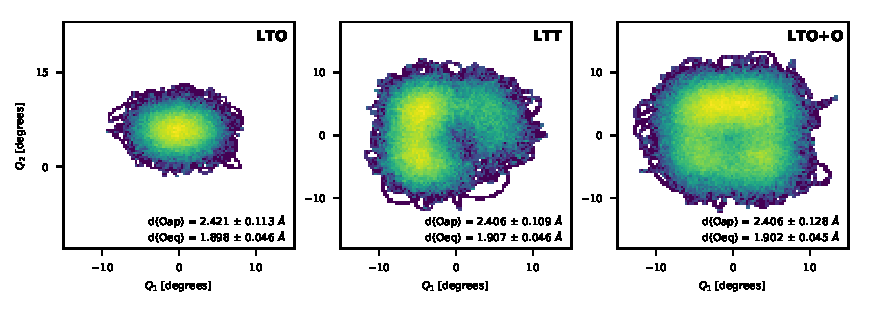
\includegraphics[width=\textwidth]{fig/md/prm_q1q2.pdf}
	\caption[MD Q1 Q2]{MD Q1 Q2}
	\label{fig:md_q1_q2}
\end{figure}

\begin{figure}
	\centering
	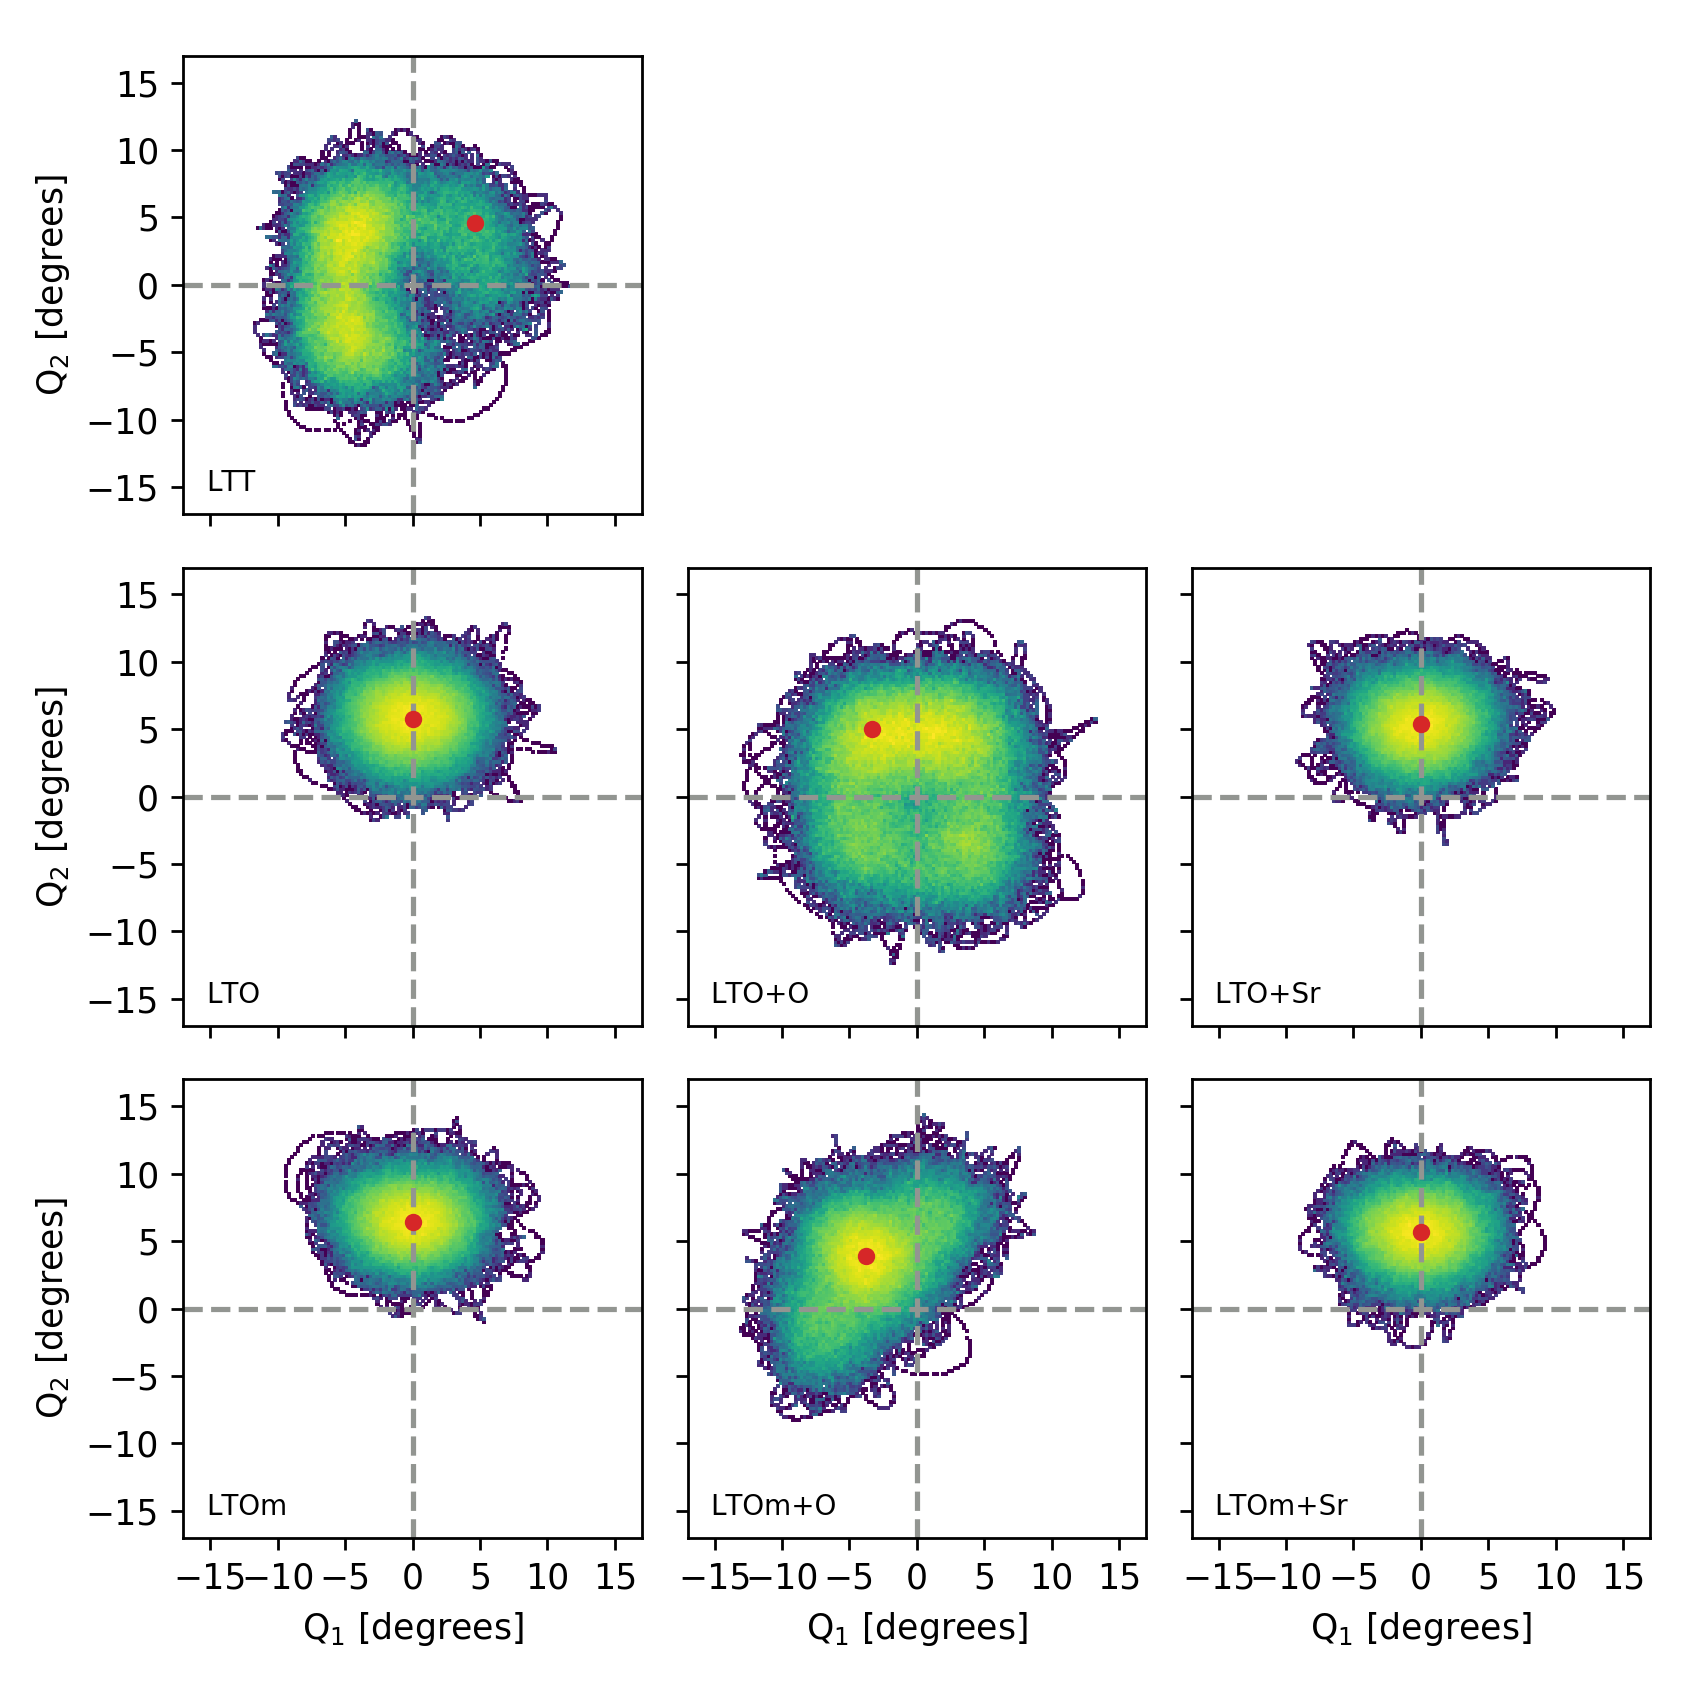
\includegraphics[width=\textwidth]{fig/md/Q1_Q2_all.png}
	\caption[MD Q1 Q2 All sims]{MD Q1 Q2 All sims}
	\label{fig:md_q1_q2_all}
\end{figure}

\begin{table}
	\centering
	\begin{tabular}{lllllll}
		\toprule
			name &   d(Oeq) & sigma(Oeq) &  R2(Oeq) &   d(Oap) & sigma(Oap) &  R2(Oap) \\
		\midrule
			 LTO &  1.89837 &  0.0454907 &  0.997277 &  2.42126 &   0.112764 &  0.998931 \\
		   LTO+O &  1.90227 &  0.0464374 &  0.997236 &  2.40559 &   0.127141 &  0.960830 \\
		  LTO+Sr &  1.89838 &  0.0507032 &  0.994707 &  2.43771 &   0.146267 &  0.999500 \\
			LTOm &  1.90897 &  0.0513818 &  0.995099 &  2.46200 &   0.140257 &  0.999679 \\
		  LTOm+O &  1.90826 &  0.0532324 &  0.993406 &  2.43961 &   0.155845 &  0.999179 \\
		 LTOm+Sr &  1.90508 &  0.0522777 &  0.994720 &  2.45116 &   0.150613 &  0.999230 \\
			 LTT &  1.90732 &  0.0460712 &  0.997086 &  2.40577 &   0.108611 &  0.999185 \\
		\bottomrule
		\end{tabular}
	\caption{MD: Cu-O Distances}
	\label{tab:md_cu_o_distances}
\end{table}

\begin{figure}
	\centering
	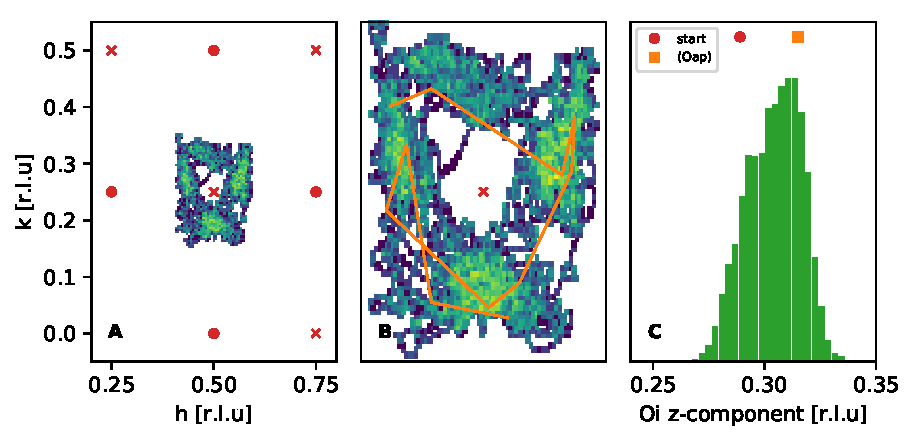
\includegraphics[width=\textwidth]{fig/md/diffusion1.pdf}
	\caption[MD Oint Diffusion Oi]{MD Oint Diffusion Oi}
	\label{fig:md_diffusion1}
\end{figure}

\begin{figure}
	\centering
	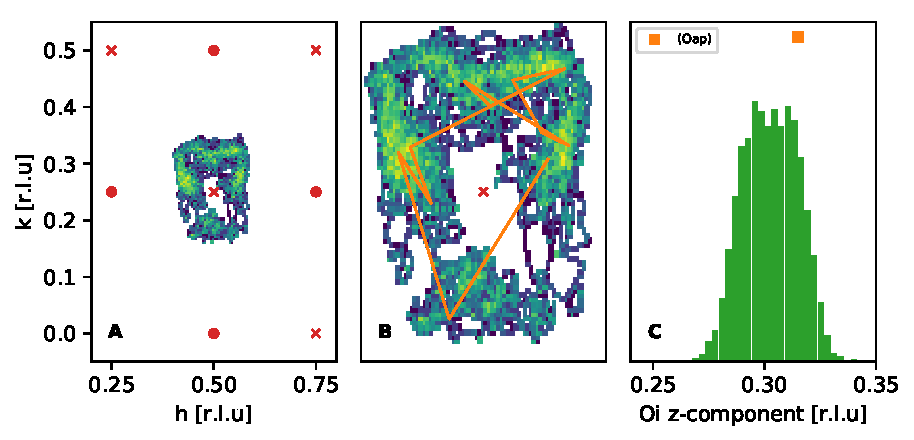
\includegraphics[width=\textwidth]{fig/md/diffusion2.pdf}
	\caption[MD Oint Diffusion Oap 1]{MD Oint Diffusion Oap 1}
	\label{fig:md_diffusion2}
\end{figure}

\begin{figure}
	\centering
	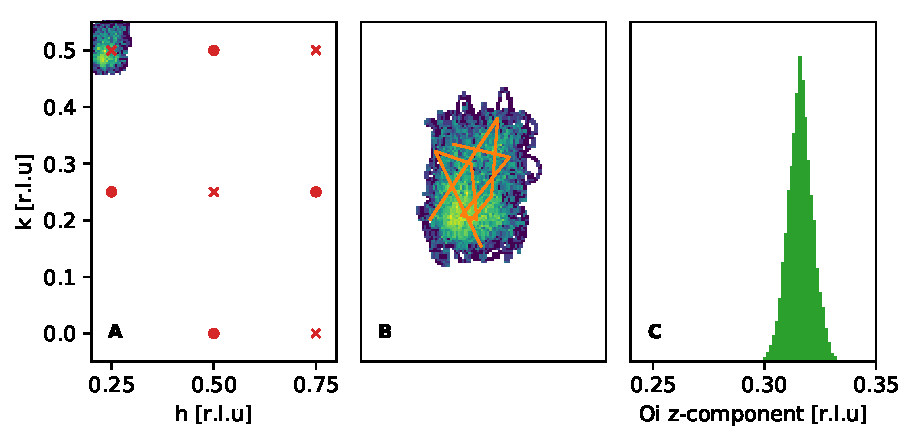
\includegraphics[width=\textwidth]{fig/md/diffusion3.pdf}
	\caption[MD Oint Diffusion Oap 2]{MD Oint Diffusion Oap 2}
	\label{fig:md_diffusion3}
\end{figure}


\begin{figure}
	\centering
	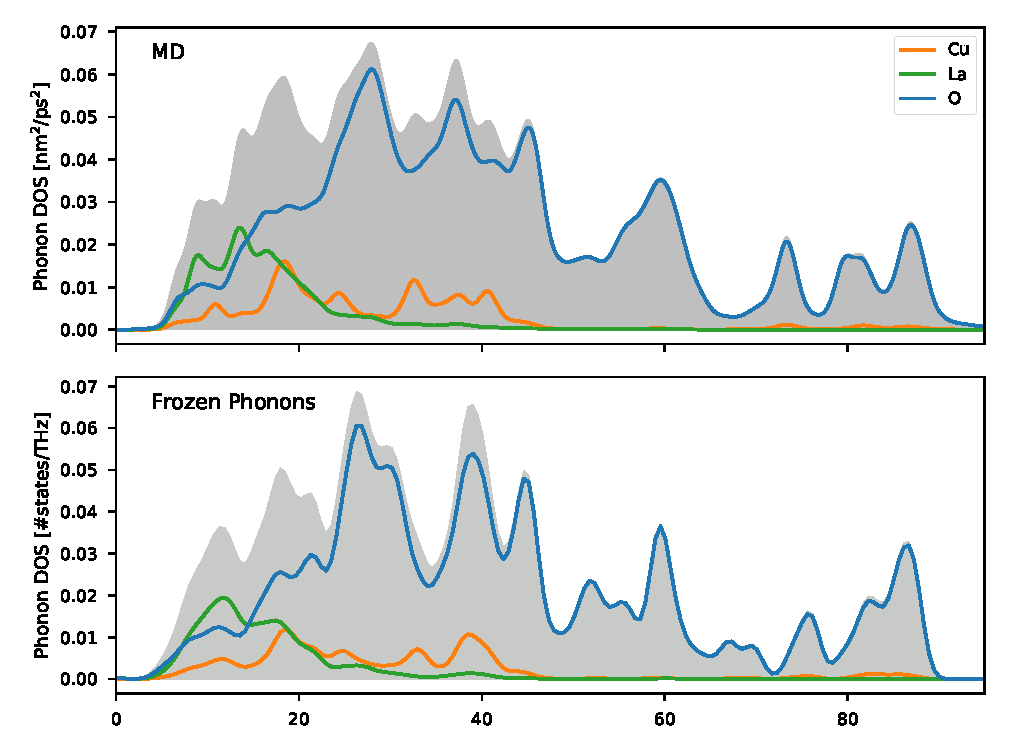
\includegraphics[width=\textwidth]{fig/md/md_phonopy_comparison.pdf}
	\caption[MD Phonopy Comparison]{MD Phonopy Comparison}
	\label{fig:md_phonopy_comparison}
\end{figure}

\section{LCO+O Phonons}
Since the introduction of interstitials breaks the local crystal symmetry, we cannot perform phonon calculations using the direct method without making an excessive amount of displacement calculations. For this reason, we are forces to use ab-initio molecular dynamics.

Before thinking about molecular dynamics, we need to place the interstitial. Figure \ref{fig:oint_location} shows possible interstitial positions for the LTO and LTT phase. We ignore the HTT phase for molecular dynamics since the symmetry is broken and, in some sense, LTT and HTT are identical (volume and a/c ratio are very similar).

\begin{figure}
    \centering
    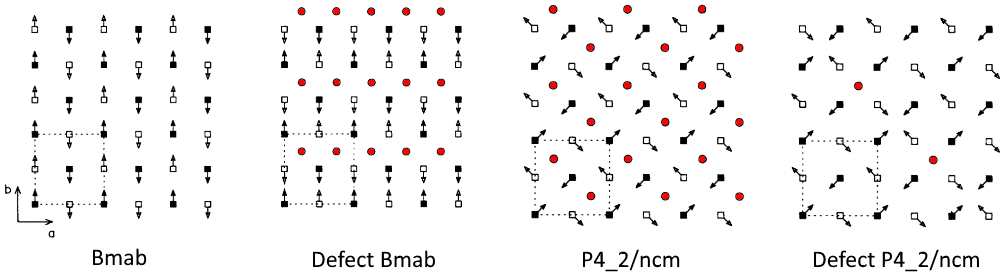
\includegraphics[width=\textwidth]{fig/md/oint.png}
    \caption[Illustration of interstitial positions]{Illustration of interstitial oxygen in-plane ($a$-$b$) location with respect to the apical oxygen displacements in the rock-salt layer. Open squares represent apical oxygens `hanging down' while closed squares represent apical oxygens `sticking up'. Interstitial oxygen are red circles. Adapted from \cite{Tranquada1995}.}
    \label{fig:oint_location}
\end{figure}

To see how the symmetry is broken, Table \ref{tab:oint_locations} shows the resulting space groups as a function of interstitial $z$-component and various defect structures in a $2 \times 2 \times 1$ supercell based on the orthorhombic crystallographic cell. 

\begin{table}[b]
    \centering
    \begin{tabular}{@{}lllll@{}}
\toprule
Phase                   & Space Group & $\text{O}_\text{i}^x$ & $\text{O}_\text{i}^y$ & $\text{O}_\text{i}^z$ \\ \midrule
HTT                     & I4/mmm (139)      &         &         &         \\
HTT + O$_\text{i}$      & P-42m  (111)    & 0.125   & 0.125   & 0.25    \\
HTT + O$_\text{i}$      & Cmm2 (35)       & 0.125   & 0.125   & 0.24    \\
LTO                     & Bmab (64)       &         &         &         \\
LTO + O$_\text{i}$      & P2 (3)    & 0.125   & 0.125   & 0.25    \\
LTO + O$_\text{i}$      & P2 (3)         & 0.125   & 0.125   & 0.24    \\
LTO$_\text{defect}$     & Pmna (53)       &         &         &         \\
LTO$_\text{defect}$ + O$_\text{i}$ & P2 (3)         & 0.875   & 0.375   & 0.25    \\
LTO$_\text{defect}$ + O$_\text{i}$ & P2 (3)         & 0.875   & 0.375   & 0.24    \\
LTT                     & P4$_2$/ncm (138)  &         &         &         \\
LTT + O$_\text{i}$      & P-4 (81)        & 0.375   & 0.125   & 0.25    \\
LTT + O$_\text{i}$      & P2 (3)         & 0.375   & 0.125   & 0.24    \\
LTT$_\text{defect}$               & Pmma (51)       &         &         &         \\
LTT$_\text{defect}$ + O$_\text{i}$ & Cmm2 (35)       & 0.875   & 0.375   & 0.25    \\
LTT$_\text{defect}$ + O$_\text{i}$ & Cmm2 (35)       & 0.875   & 0.375   & 0.24    \\ \bottomrule
\end{tabular}

    \caption[Oxygen interstitial phases]{Space group symmetry due to the introduction of an interstitial oxygen in various structures all described in a $2 \times 2 \times 1$ supercell of the Bmab (conventional) coordinate system. HTT, LTO and LTT are the usual phases as described in litterature \cite{Hucker2012}. The structures labeled defect is (A) in the LTO case: A stacking fault where the middle layer has its tilts reversed and (B) in the LTT case: A line along [110] with reversed tilts. Both are described in \cite{Tranquada1994} and are designed in order to `make room' for the interstitial oxygen (see Figure \ref{fig:oint_location}).}
    \label{tab:oint_locations}
\end{table}

We performed high-precision geometry optimizations (with symmetry turned off) on these structures (including a test of HTT) resulting in the table of energies as shown in Table \ref{tab:oint_en}. While the defect structures intuitively would make more room for oxygen interstitials, the energy cost of forming the defect is higher in the, relatively small, supercell that we use. It is worth noting, however, that they move to very similar energies during the optimization\todo{not so surprising, since they probably move towards the same structure. I need to check this more closely}.


\begin{table}[b]
    \centering
    \begin{tabular}{@{}lll@{}}
    \toprule
     & $E_0$ [eV] & $E_1$ [eV]            \\ \midrule
    HTT                     & -827.27669             & -829.76250 \\
    LTO                     & -828.29890             & -830.39658 \\
    LTO\_sfault              & -823.09516             & -830.03588 \\
    LTT                     & -828.04663             & -830.08248 \\
    LTT\_defect              & -826.03173             & -829.94243 \\ \bottomrule
    \end{tabular}
    \caption[Oxygen interstital phases: Energy]{Oxygen interstital phases: Energy. $E_0$ corresponds to the energy after inserting the interstitial oxygen, but before geometry optimization. $E_1$ is the total energy after optimization. Geomtry optimization performed on ionic positions only. Conclusion: It costs more energy to create the defect structure than you gain by making room for the interstitial.}
    \label{tab:oint_en}
\end{table}